% !TeX spellcheck = en_US

\chapter{Add new package manager module}\label{chap:add}
This chapter will show extensibility of framework by adding new package manager module for $aptitude$ package manager.\\
Section \ref{sec:aptitude} provides common information about the package manager.\\
In section \ref{sec:aptitude_imp} module is implemented and in section \ref{sec:aptitude_int} is integrated into bash language module

\section{Aptitude}\label{sec:aptitude}
This section describes the $aptitude$ package manager.
Like $apt$-$get$ is $aptitude$ command line program and just like the $apt$-$get$ a package can be installed using command $aptitude$ $install$ \emph{package}. In additional it can be started in pseudo-graphic mode, to provide visual interface (figure \ref{fig:aptitude_gui}).
\begin{figure}[ht]   
	\centering
	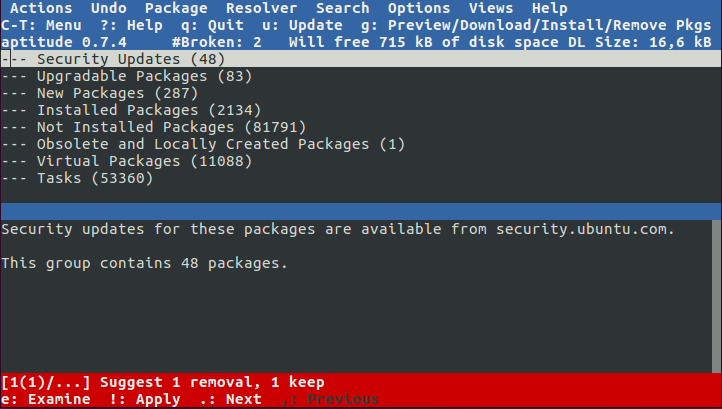
\includegraphics[width=0.7\textwidth]{Screenshot_aptitude.png}
	\caption{Command line visual interface for $aptitude$ package manager.}
	\label{fig:aptitude_gui}
\end{figure}
Another additional capability compared to $apt$-$get$ is a search for packages by a part of the name (or by other attributes) using the $aptitude$ $search$ command.
\section{Implementing new package manager module}\label{sec:aptitude_imp}
\section{Integrating Aptitude into Bash module}\label{sec:aptitude_int}